\section{Literature Review}
\label{sec:Lit}

Figure~\ref{fig:litmap} summarises how the sources in the research bibliography relate to conceptual themes. Branches group survey, runtime verification, automotive and trust, and methods/tooling; each citation is paired with a short summary (no duplicated sources).

% Single-column literature map (fits IEEE column width).
\begin{figure}[!t]
  \centering
  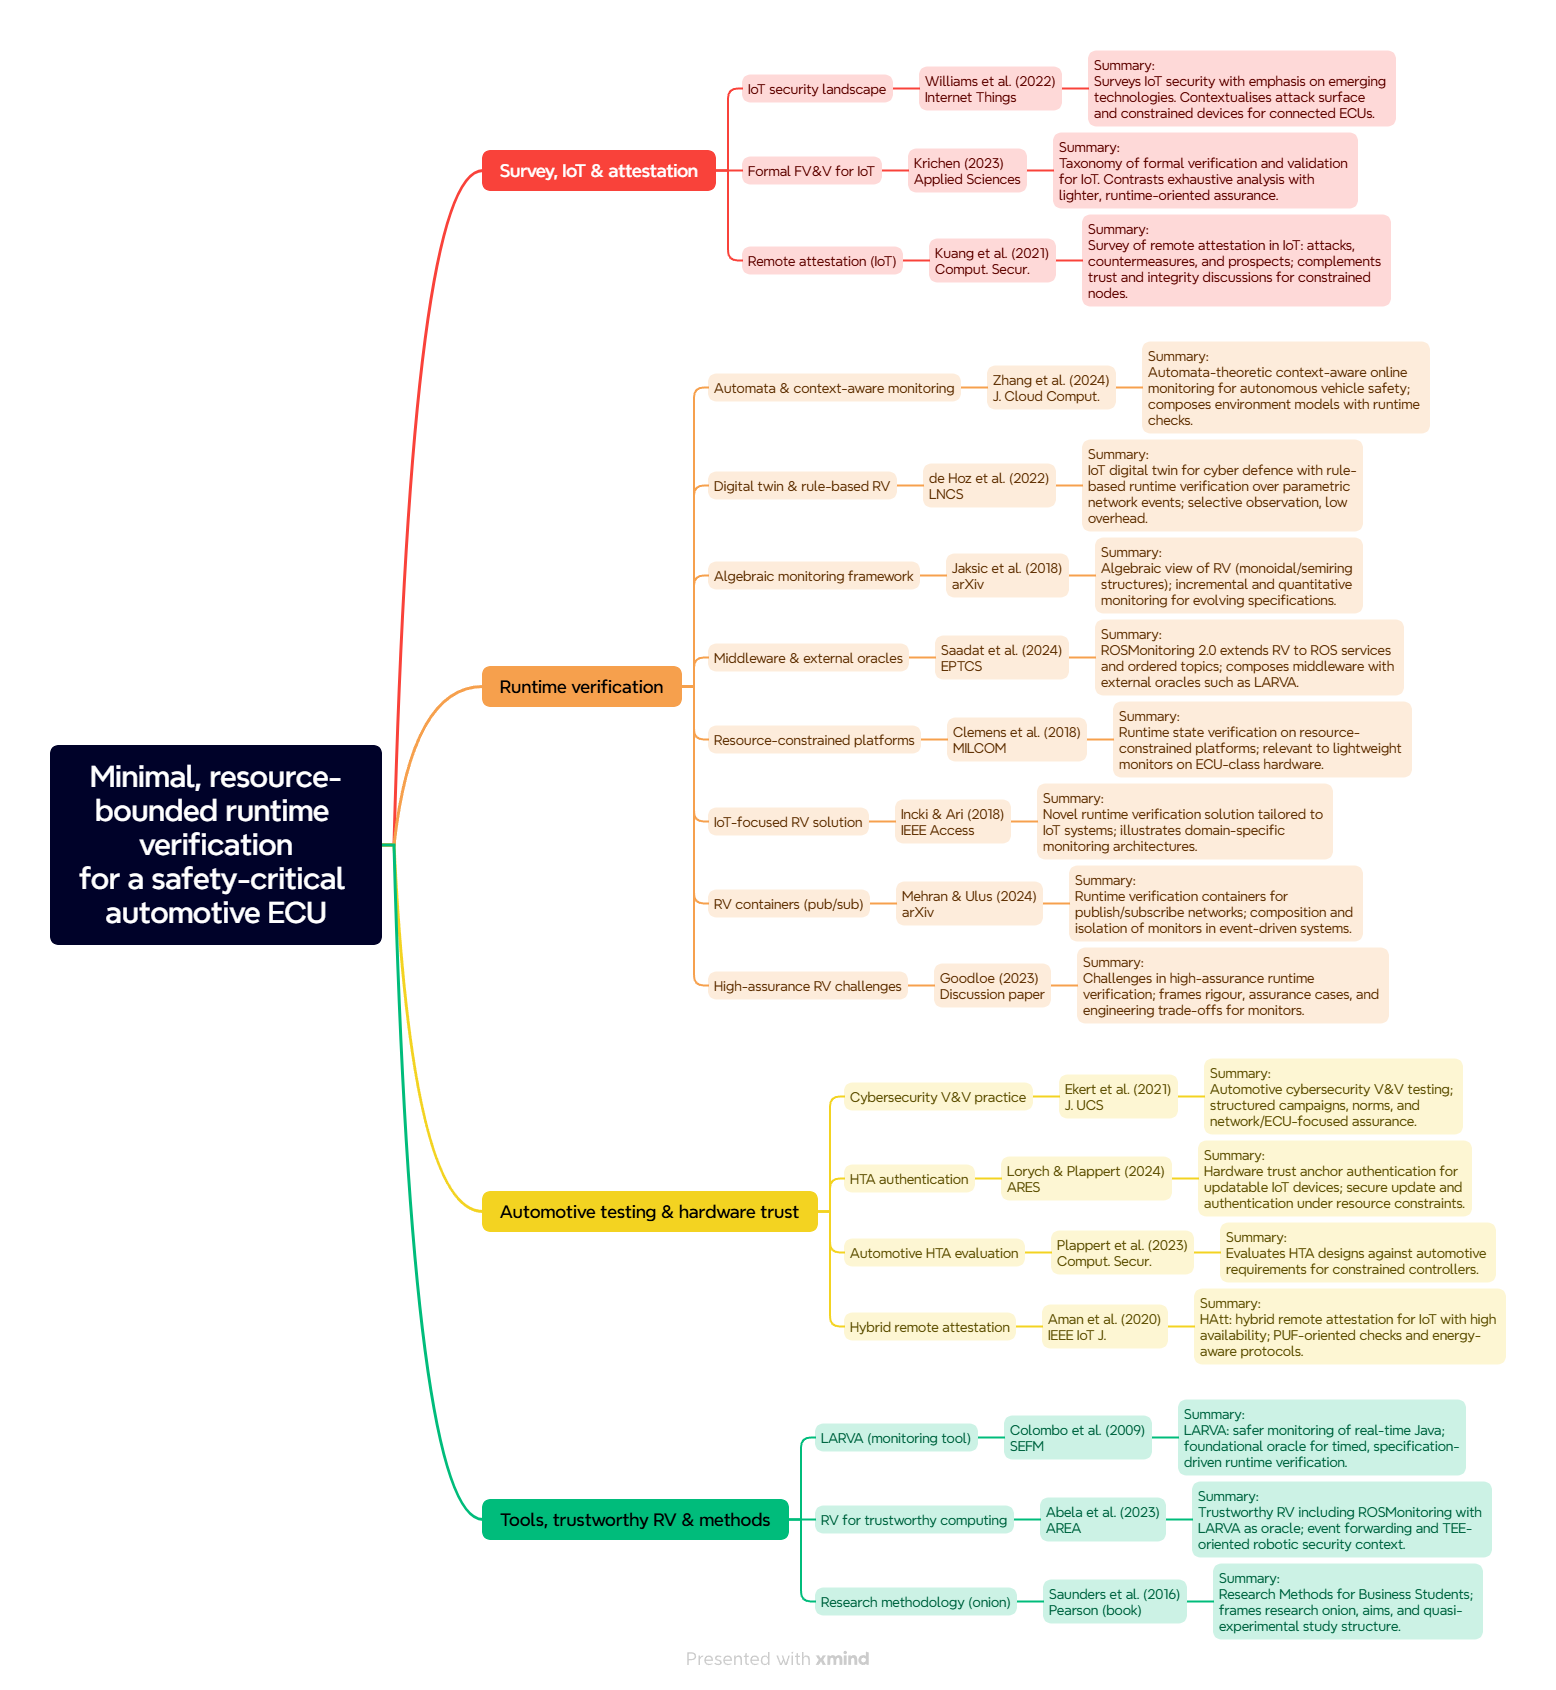
\includegraphics[width=\columnwidth]{figures/LiteratureMap.png}%
  \caption{Literature map covering the full research bibliography (survey/IoT/attestation; runtime verification; automotive testing and hardware trust; tools, trustworthy RV, and methodology). Each citation is paired with a short summary. Sources: Williams \textit{et al.}~\cite{williams2022survey}, Krichen~\cite{krichen2023survey}, Kuang \textit{et al.}~\cite{kuang2021remote}, Zhang \textit{et al.}~\cite{zhang2024context}, de Hoz Diego \textit{et al.}~\cite{dehoz2022iotdt}, Jak\v{s}i\'c \textit{et al.}~\cite{jaksic2018algebraic}, Saadat \textit{et al.}~\cite{saadat2024rosmonitoring2}, Clemens \textit{et al.}~\cite{clemens2018runtime}, Incki and Ari~\cite{incki2018novel}, Mehran and Ulus~\cite{mehran2024containers}, Goodloe~\cite{goodloe2023highassurance}, Ekert \textit{et al.}~\cite{ekert2021cybersecurity}, Lorych and Plappert~\cite{lorych2024hta}, Plappert \textit{et al.}~\cite{plappert2023hta}, Aman \textit{et al.}~\cite{aman2020hatt}, Colombo \textit{et al.}~\cite{colombo2009larva}, Abela \textit{et al.}~\cite{abela2023rvtee}, Saunders \textit{et al.}~\cite{saunders2016research}.}
  \label{fig:litmap}
\end{figure}


This section reviews how recent studies approach verification, monitoring, and trust for connected, resource-constrained controllers such as automotive ECUs and IoT devices. The discussion is grounded in the sources charted in Fig.~\ref{fig:litmap}~\cite{williams2022survey,krichen2023survey,kuang2021remote,zhang2024context,dehoz2022iotdt,jaksic2018algebraic,saadat2024rosmonitoring2,clemens2018runtime,incki2018novel,mehran2024containers,goodloe2023highassurance,ekert2021cybersecurity,lorych2024hta,plappert2023hta,aman2020hatt,colombo2009larva,abela2023rvtee,saunders2016research}.

\subsection{Methodological themes in related work}

Related work clusters into five strands: (i) surveys/taxonomies of IoT FV\&V and security constraints~\cite{krichen2023survey,williams2022survey}; (ii) automotive cybersecurity V\&V practice~\cite{ekert2021cybersecurity}; (iii) runtime monitoring formalisms and context-aware detection~\cite{zhang2024context,dehoz2022iotdt,jaksic2018algebraic}; (iv) tool-chain integration studies such as ROSMonitoring~2.0~\cite{saadat2024rosmonitoring2}; and (v) trust-anchor and attestation mechanisms relevant to constrained devices~\cite{plappert2023hta,lorych2024hta,aman2020hatt}.

\subsection{Source quality note}

\textbf{Academic} sources here include peer-reviewed journals (e.g.~\cite{ekert2021cybersecurity,williams2022survey,plappert2023hta,zhang2024context,krichen2023survey}), archival conference proceedings (e.g.~\cite{lorych2024hta}), and edited volume chapters (e.g.~\cite{dehoz2022iotdt}). Workshop and electronic proceedings such as EPTCS~\cite{saadat2024rosmonitoring2} are scholarly but differ from flagship journals in review depth and indexing. This review therefore prioritises peer-reviewed evidence while using conference and workshop material where it contributes directly to implementation context.
By contrast, \textbf{non-academic} material (e.g., blogs, promotional vendor pages, and informal forum posts) is excluded from evidential claims and used, if at all, only for implementation context rather than as primary support for arguments.

\subsection{Five recommended peer-reviewed journal articles}

For readers prioritising archival journal literature, five papers are especially relevant: (1)~Ekert \textit{et al.}~\cite{ekert2021cybersecurity} on automotive cybersecurity V\&V testing; (2)~Krichen~\cite{krichen2023survey} on FV\&V for IoT; (3)~Williams \textit{et al.}~\cite{williams2022survey} on IoT security and emerging technologies; (4)~Plappert \textit{et al.}~\cite{plappert2023hta} on hardware trust anchors in automotive settings; and (5)~Zhang \textit{et al.}~\cite{zhang2024context} on automata-theoretic, context-aware monitoring for autonomous vehicle safety. Together they cover testing practice, formal-method surveys, the security landscape, trust hardware, and concrete monitoring formalisms.

\subsection{Contextualisation for this study}

This project adopts a minimal ECU-focused monitor design informed by those strands: automotive testing context from Ekert~\cite{ekert2021cybersecurity}, constrained-security framing from Williams~\cite{williams2022survey}, monitor formalisation from Zhang/de Hoz/Jak\v{s}i\'c~\cite{zhang2024context,dehoz2022iotdt,jaksic2018algebraic}, and trust-extension pathways from HTA/attestation work~\cite{plappert2023hta,lorych2024hta}.

\subsection{Critical comparison and knowledge gaps}

The literature does not fully provide a reproducible, ECU-local, lightweight RV pipeline with direct ON/OFF overhead measurements under controlled abnormal injections. Three practical gaps motivate this study: (i) monitor-set selection for constrained ECU traces, (ii) threshold calibration under safety/security trade-offs, and (iii) explicit overhead attribution in violation-heavy execution paths.
